
\documentclass{article}
\usepackage{tikz}
\pagestyle{empty}
\makeatletter
\def\dt@pt#1{#1\typeout{PT \the\pgf@x,\the\pgf@y}}
\let\dt@move\pgfpathmoveto
\def\pgfpathmoveto#1{\dt@pt{#1}\typeout{MOVE}\dt@move{#1}}
\let\dt@curve\pgfpathcurveto
\def\pgfpathcurveto#1#2#3{\dt@pt{#1}\dt@pt{#2}\dt@pt{#3}\typeout{CURVE}\dt@curve{#1}{#2}{#3}}
\makeatother
\begin{document}
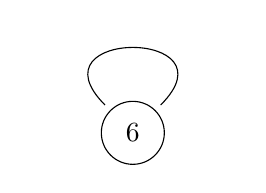
\begin{tikzpicture}[x=1cm,y=1cm]
\node[circle,draw,outer sep=1mm,minimum size=8mm] (six) at (0,0) {$6$}; \draw (six) to[out=135,in=45,looseness=5] (six);
\end{tikzpicture}
\end{document}
